\documentclass[20pt,,margin=1in,innermargin=-4.5in,blockverticalspace=-0.25in]{tikzposter}
\geometry{paperwidth=42in,paperheight=36in}
\usepackage[utf8]{inputenc}
\usepackage{amsmath}
\usepackage{amsfonts}
\usepackage{amsthm}
\usepackage{amssymb}
\usepackage{mathrsfs}
\usepackage{graphicx}
\usepackage{adjustbox}
\usepackage{enumitem}
\usepackage{braket}
\usepackage[backend=biber,style=numeric]{biblatex}
\usepackage{SUtheme}

\usepackage{mwe} % for placeholder images

\addbibresource{refs.bib}

% set theme parameters
\tikzposterlatexaffectionproofoff
\usetheme{SUTheme}
\usecolorstyle{SUStyle}
\usetitlestyle{Filled}

\usepackage[scaled]{helvet}
\renewcommand\familydefault{\sfdefault} 
\usepackage[T1]{fontenc}


\title{Topological Quantum Computing}
\author{Turner Entenmann, Hunter Hamby, John Hawthorne}
\institute{University of Wisconsin}
\titlegraphic{
\includegraphics[width=0.04\textwidth]{logo/red-UWcrest-print.eps}}

% begin document
\begin{document}
\maketitle
\centering
\begin{columns}
    \column{0.32}
    \block{Introduction}{
        \begin{itemize}
            \item There are several ways to do quantum computing. This presentation will focus on topological quantum computing. 
            \item Topological quantum computing uses quasiparticles called anyons as qubits. 
            \item The logic gates in topological quantum computing are called braids. Braids are used in topology and act as transformations between particles.
            \item While topological quantum computing is still highly theoretical, some people have already presented possible real life implementations. 
            \item Topological quantum computing is of interest since it is inherently error resistant. Topology is only worried about global properties of the system and thus is resistant to local perturbations.
        \end{itemize}
    }
    \block{Qubits - Anyons}{
        \begin{itemize}
            \item All particles in 3D are either Bosons (photons, gluons, $\ldots$) or Fermions (electrons, protons, $\ldots$) depending on how they behave under particle exchange. Bosons are symmetric: $\psi(\Vec{r}_1,\Vec{r}_2)=\psi(\Vec{r}_2,\Vec{r}_1)$ and Fermions are anti-symmetric: $\psi(\Vec{r}_1,\Vec{r}_2)=-\psi(\Vec{r}_2,\Vec{r}_1)$
            \item Double adiabatic interchange of particles is physically the same as one particle traveling around the other. In 3D this is topologically the same as as neither particle moving because the path of the moving particle can be pulled around the stationary one and closed to a point
        \end{itemize}
        \begin{tikzfigure}[3D vs 2D topology of double exchange \cite{cite:1}]
            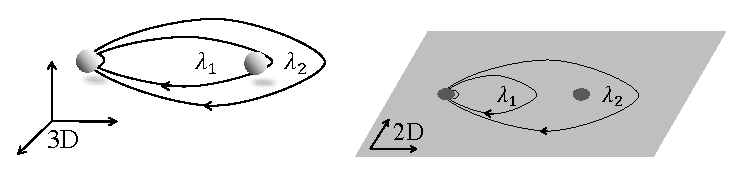
\includegraphics[width=0.9\linewidth]{Images/2d3d.pdf}
        \end{tikzfigure}
        \begin{itemize}
            \item In 2D the path of one particle traveling around another cannot be closed without being cut. Therefore, one particle traveling around another is topologically distinct from both particles remaining stationary
             \item In this situation the interchange of particles introduces a phase $\theta$ that is not necessarily $0$ or $\pi$
             \item Particles with such $\theta$ are called "anyons"
             \item While there have been a handful of methods proposed (only some of which can be used to make a universal quantum computer), actually creating and manipulating anyons remains extremely difficult and most of the work in this area remains theoretical.
             \item One of the most promising ways of generating anyons using the fractional quantum Hall effect.
             \item The fractional quantum Hall effect comes from the classical Hall effect having quantized states that are not integer value.
             \item Anyons are excitations of the ground state of the the fractional quantum Hall state.
             \item While non-Abelian anyons have not been observed, this is currently the leading area of research to observe them.
             \item Assuming that anyons exist and can be sufficiently isolated from the environment there are three operations that can be performed \cite{cite:1}
             \begin{itemize}
                 \item Pairwise creation and annihilation
                 \item Pairwise fusion forming different types of anyons
                 \item Adiabatic exchange
             \end{itemize}
             \item These operations allow us to construct qubits which we can entangle, manipulate and measure
         \end{itemize}
    }
   
    \column{0.36}
    \block{Braids \& Logic Gates}{


        \begin{tikzfigure}[The elementary braids corresponding to $X$, $Z$ Hadamard and controlled $Z$ in the Ising model \cite{cite:1}]
            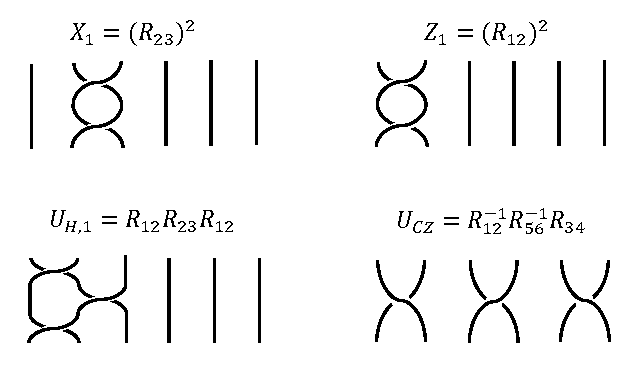
\includegraphics[width=0.5\linewidth]{Images/Ising_braids.pdf}
        \end{tikzfigure}
    }

    \column{0.32}
    \block{Implementation}{
        \begin{center}
            \textbf{\underline{Fibonacci Anyons} \cite{cite:1}}
        \end{center}
        \begin{itemize}
            \item One possible method of implementing a topological computer is using Fibonacci anyons
            \item Fibonacci anyons are the simplest non-Abelian anyon, there is only one anyon $\tau$ which is its own anti-particle and two $\tau$ anyons can behave like a single $\tau$ anyon. The fusion rule is
        \end{itemize}
        \begin{gather*}
            \tau\times\tau=1+\tau
        \end{gather*}
        \begin{itemize}
            \item Repeated associative application of the fusion rule shows the number of different ways the fusion can result in either the vacuum $1$ or the anyon $\tau$
        \end{itemize}
        \begin{align*}
            \tau\times\tau\times\tau&=1+2\cdot\tau\\
            \tau\times\tau\times\tau\times\tau&=2\cdot1+3\cdot\tau\\
            \tau\times\tau\times\tau\times\tau\times\tau&=3\cdot1+5\cdot\tau\\
        \end{align*}
        \begin{itemize}
            \item The encoding requires three $\tau$ anyons constrained to fuse to a single $\tau$ particle
            \item A basis in this situation is $\ket{(\tau\tau)\tau;1\tau;\tau}$ and $\ket{(\tau\tau)\tau;\tau\tau:\tau}$
            \item The fusion and braiding matrices are then $\left(\phi=\frac{1+\sqrt{5}}{2}\right)$
        \end{itemize}
        \begin{align*}
            F&=\begin{pmatrix}
                \phi^{-1}&\phi^{-1/2}\\\phi^{-1/2}&\phi^{-1}
            \end{pmatrix}&
            R&=\begin{pmatrix}
                e^{\frac{4\pi i}{5}}&0\\0&e^{\frac{-3\pi i}{5}}
            \end{pmatrix}
        \end{align*}
        \begin{itemize}
            \item Because $F^{-1}RF$ is dense in $SU(2)$, any single qubit gate can be approximated to arbitrary accuracy
            \item This would seem to make Fibonacci anyons an obvious choice for topological quantum computing, unfortunately, there are two major problems
            \begin{itemize}
                \item Fibonacci anyons lack a tensor product, therefore only a subspace of the full fusion space can be used to encode information.
                \item The other problem is that approximating gates requires many braids. For example, the $NOT$ gate requires thousands of braids
            \end{itemize}
            \item There is no practical implementation of Fibonacci anyons (yet)
        \end{itemize}
        \begin{center}
            \textbf{\underline{Ising Anyons} \cite{cite:1}}
        \end{center}
        \begin{itemize}
            \item The Ising anyon model consists of two non-trivial particles $\psi$ a fermion and $\sigma$ an anyon together with the vacuum $1$.
            \item They obey the fusion rules
        \end{itemize}
        \begin{align*}
            1\times1&=1 & 1\times\psi&=\psi & 1\times\sigma=\sigma\\
            \psi\times\psi&=1 & \psi\times\sigma&=\sigma & \sigma\times\sigma&=1+\psi
        \end{align*}
        \begin{itemize}
            \item These rules give raise to the following fusion and braiding matrices:
        \end{itemize}
        \begin{align*}
            F&=\frac{1}{\sqrt{2}}
            \begin{pmatrix}
                1&1\\1&-1
            \end{pmatrix} & R&=e^{-i\frac{\pi}{8}}
            \begin{pmatrix}
                1&0\\0&e^{i\frac{\pi}{2}}
            \end{pmatrix}
        \end{align*}
        \begin{itemize}
            \item Unfortunately, no combination of $F$ and $R$ are dense in $SU(2)$ so Ising anyons cannot make a universal quantum computer. They can however, implement the Clifford group and so has some utility
        \end{itemize}
    }
    
    \block{References}{
        \vspace{-1em}
        \begin{footnotesize}
        \printbibliography[heading=none]
        \end{footnotesize}
    }
\end{columns}
\end{document}
